%%
%% ACM RecSys 2026 — MACS Merchant Agent Paper
%% [Author and institution details omitted for blind review]
%%
\documentclass[sigconf,anonymous]{acmart}

\AtBeginDocument{%
  \providecommand\BibTeX{{Bib\TeX}}}

\setcopyright{acmlicensed}
\copyrightyear{2026}
\acmYear{2026}
\acmDOI{XXXXXXX.XXXXXXX}
\acmConference[RecSys '26]{ACM Conference on Recommender Systems}{September 28--October 2, 2026}{Minneapolis, Minnesota, USA}
\acmISBN{978-1-4503-XXXX-X/26/09}

\usepackage{tikz}
\usetikzlibrary{positioning,arrows.meta,fit,shadows,calc}
\usepackage{algorithm}
\usepackage{algpseudocode}
%% microtype loaded by acmart — do not re-load (causes \showhyphens warning)
\usepackage{graphicx}
\usepackage{booktabs}
\usepackage{enumitem}
\citestyle{acmauthoryear}
%% Give LaTeX extra stretch budget to avoid overfull hboxes
\emergencystretch=1.5em
%% Allow line breaks around the + in catalog-bound system names
\newcommand{\GPTCatalog}{GPT\allowbreak{}+\allowbreak{}Catalog}
\newcommand{\GeminiCatalog}{Gemini\allowbreak{}+\allowbreak{}Catalog}

\begin{document}

\title[Reliable Conversational Recommendation for Agentic E-Commerce]{
MACS: A Hybrid Merchant-Agent Framework for Reliable Conversational E-Commerce Recommendation
}

%% ---- BLIND REVIEW VERSION ----
%% Author information suppressed per double-blind review policy.
%%
%% CAMERA-READY TODO: uncomment the full author block below and DELETE the
%% Anonymous Author block that follows it.
%% CAMERA-READY TODO: in \begin{acks} near the end, replace
%%   "[details omitted for blind review]" with the full acknowledgment text.
%%
%% \author{Juli Huang}
%% \affiliation{%
%%   \institution{Stanford University}
%%   \department{Department of Computer Science}
%%   \city{Stanford}\state{CA}\country{USA}}
%% \email{julih@stanford.edu}
%%
%% \author{Hannah Clay}
%% \affiliation{%
%%   \institution{Stanford University}
%%   \department{Department of Computer Science and Biocomputation Program}
%%   \city{Stanford}\state{CA}\country{USA}}
%% \email{hclay@stanford.edu}
%%
%% \author{Thomas Sarda}
%% \affiliation{%
%%   \institution{Stanford University}
%%   \department{Department of Management Science \& Engineering}
%%   \city{Stanford}\state{CA}\country{USA}}
%% \email{tsarda@stanford.edu}
%%
%% \author{Sajjad Beygi}
%% \affiliation{%
%%   \institution{Stanford University}
%%   \department{Department of Electrical Engineering}
%%   \city{Stanford}\state{CA}\country{USA}}
%% \email{beygi@stanford.edu}
%%
%% \renewcommand{\shortauthors}{Huang et al.}
\author{Anonymous Author(s)}
\affiliation{%
  \institution{Anonymous Institution}
  \city{Anonymous City}
  \country{Anonymous Country}}
\renewcommand{\shortauthors}{Anonymous et al.}

\begin{abstract}
Conversational recommendation for e-commerce is increasingly mediated by large language models (LLMs), but many real-world deployments operate under a stricter requirement: recommendations must be drawn only from a merchant’s fixed catalog, without web search or unsupported product claims. In this setting, the central challenge is reliability under hard constraints: the system must satisfy user requirements, remain grounded in available inventory, and preserve preferences across multiple conversational turns.

We present MACS (Merchant Agent Commerce System), a hybrid merchant-agent framework for reliable conversational recommendation in fixed-catalog settings. MACS separates natural-language interaction from correctness-critical enforcement within the merchant agent: deterministic components handle hard-constraint filtering, brand exclusion, progressive relaxation, and reasoning over structured product relations, while LLMs are used for natural-language understanding and response generation. A session-persistent preference layer tracks and updates user constraints across turns, enabling consistent handling of conversational state changes such as budget overwrites and exclusion reversals.
Beyond recommendation, MACS supports product comparison, add-to-cart, checkout, and service queries through a unified backend compatible with emerging agent-commerce protocols. Evaluations on single-turn and multi-turn benchmarks show that MACS achieves the strongest reliability among the evaluated catalog-constrained systems. On a single-turn benchmark, MACS achieves the highest pass rate and perfect brand compliance. On a multi-turn benchmark, MACS achieves 100\% Pass@5 on the hardest
state-management scenario---exclusion reversal---where prompt-based baselines
score only 20\% (\GPTCatalog{}) and 0\% (\GeminiCatalog{}). MACS also
achieves 100\% Pass@5 on budget overwrite, matching \GeminiCatalog{} and
outperforming \GPTCatalog{} (80\%).

On multi-turn macro Pass@5, MACS leads all systems (60\% vs.\ 54\% \GPTCatalog{} vs.\ 52\% \GeminiCatalog{}), with zero constraint drift. These results show that reliable conversational
recommendation in merchant-controlled catalogs is best supported by hybrid
architectures that combine LLM-based interaction with deterministic constraint
enforcement and explicit preference tracking.

\end{abstract}

\begin{CCSXML}
<ccs2012>
 <concept>
  <concept_id>10002951.10003317.10003347.10003350</concept_id>
  <concept_desc>Information systems~Recommender systems</concept_desc>
  <concept_significance>500</concept_significance>
 </concept>
 <concept>
  <concept_id>10002951.10003317.10003371.10003386</concept_id>
  <concept_desc>Information systems~Question answering</concept_desc>
  <concept_significance>300</concept_significance>
 </concept>
 <concept>
  <concept_id>10010147.10010257.10010293.10010294</concept_id>
  <concept_desc>Computing methodologies~Multi-agent systems</concept_desc>
  <concept_significance>300</concept_significance>
 </concept>
 <concept>
  <concept_id>10002951.10003317.10003347.10003360</concept_id>
  <concept_desc>Information systems~Social networks</concept_desc>
  <concept_significance>100</concept_significance>
 </concept>
</ccs2012>
\end{CCSXML}

\ccsdesc[500]{Information systems~Recommender systems}
\ccsdesc[300]{Information systems~Question answering}
\ccsdesc[300]{Computing methodologies~Multi-agent systems}
\ccsdesc[100]{Information systems~Social networks}

\keywords{limited-catalog shopping, reliability, conversational recommendation,
agentic commerce, multi-agent systems, knowledge graph reasoning,
preference elicitation, constraint enforcement, Model Context Protocol,
Universal Commerce Protocol, semantic search}

\maketitle

%% ==========================================================================

\section{Introduction}
\label{sec:introduction}

Conversational recommender systems increasingly rely on large language models
(LLMs) to interact with users in natural language, elicit preferences, and
generate recommendations. A particularly important and underexplored deployment
setting is \emph{limited-catalog shopping}: a merchant agent operating over its
own fixed product database, with web search disabled, that must recommend only
from verified inventory while respecting user constraints. This setting gives
merchants control over product data and avoids the latency and hallucination
risks of web-augmented search, but it also places strict reliability demands on
the recommender. LLMs, despite their fluency, remain unreliable in this setting:
they may hallucinate product specifications not present in the catalog, forget
earlier brand exclusions across turns, or apply budget filters inconsistently.
A recommender that returns out-of-catalog products or violates a user's stated
constraints fails a core reliability requirement.

We present \textbf{MACS (Merchant Agent Commerce System)}, a hybrid
merchant-agent framework for reliable conversational recommendation in
fixed-catalog settings. Unlike classical e-commerce APIs that require
structured query parameters, MACS accepts natural-language input directly:
the merchant agent's interface can be driven by free-text queries from a
shopping agent or a user, while all constraint enforcement remains
deterministic internally. MACS separates natural-language interaction from
correctness-critical enforcement: the LLM handles preference elicitation
and response generation, while constraint filtering, brand exclusion, and
cross-turn preference persistence are delegated to structured, auditable
components. This design allows the system to support natural multi-turn
interactions without sacrificing catalog grounding or deterministic
constraint correctness.

The evaluation shows that this architectural separation matters. On the shared
single-turn benchmark, MACS achieves the highest pass rate and perfect brand and
filter compliance. On a 10-scenario multi-turn benchmark, MACS leads all systems
on macro Pass@5 (60\% vs.\ 54\% \GPTCatalog{} vs.\ 52\% \GeminiCatalog{}) with
mean score 0.739 (vs.\ 0.747 GPT / 0.727 Gemini, within one SD); MACS uniquely achieves 100\% Pass@5
on exclusion reversal---the scenario requiring mid-session state
updates---where \GPTCatalog{} scores 20\% and \GeminiCatalog{} scores 0\%.
These results indicate that reliable conversational recommendation in
merchant-controlled catalogs benefits from hybrid architectures that combine
LLM-based interaction with deterministic constraint enforcement and explicit
preference tracking. We make three contributions:
\begin{itemize}[leftmargin=*]
    \item We propose a hybrid merchant-agent architecture that separates
    LLM-based natural-language interaction from deterministic constraint
    enforcement, enabling reliable product recommendation over a fixed,
    merchant-owned catalog without web search.

    \item We introduce session-persistent preference state management that
    preserves user constraints across turns, supports updates such as budget
    overwrites and exclusion reversals, and enables consistent multi-turn
    recommendation behavior.

    \item We present a hybrid evaluation framework that separates deterministic
    constraint correctness from response quality, enabling faithful assessment
    of conversational recommenders in both single-turn and multi-turn
    limited-catalog settings.
\end{itemize}

MACS is also deployed in an \emph{agent-to-agent e-commerce} setting, in which
shopping agents interact with merchant agents through structured interfaces.
To support this, a single backend exposes three agent-commerce
protocols---Model Context Protocol (MCP)~\cite{Anthropic2024MCP},
Universal Commerce Protocol (UCP)~\cite{Google2026UCP},
and Agent Commerce Protocol (ACP)~\cite{OpenAI2025ACP}---with no
per-protocol application logic.
This protocol layer is a deployment feature; the core contribution of the paper
is the reliability framework for limited-catalog conversational recommendation.

%% ==========================================================================
\section{Related Work}
%% ==========================================================================

\paragraph{Conversational Recommender Systems.}
CRSs elicit user preferences through multi-turn interaction~\cite{Jannach2021Survey},
ranging from bandit-based question selection~\cite{Christakopoulou2016,Sun2018}
to LLM-integrated pipelines for preference understanding and response
generation~\cite{Friedman2023,Feng2023LLMCRS,Liu2023CRSLLM}.
Retrieval augmentation~\cite{Yang2024ReFICR}, cross-session
memory~\cite{Xi2024MemoCRS}, and behavioral evaluation~\cite{Yang2024BehaviorAlignment}
have further extended the paradigm.
MACS addresses a gap these works leave open: deterministic enforcement of
hard user constraints (excluded brands, budget ceilings, spec minimums)
across turns, without relying on LLM faithfulness.

\paragraph{Knowledge Graphs and LLM Agents for Shopping.}
Knowledge-aware recommenders (CKE~\cite{Zhang2016CKE}, KGCN~\cite{Wang2019KGCN},
KGAT~\cite{Wang2019KGAT}) incorporate graph structure into learned representations;
MACS uses a knowledge graph operationally for structural queries (substitutes,
compatibility) with auditable Cypher traversal rather than learned embeddings.
Shopping-agent benchmarks (WebArena~\cite{Zhou2023WebArena},
AgentBench~\cite{Liu2023AgentBench}, ShoppingBench~\cite{Wang2025ShoppingBench})
study the \emph{shopping-agent} side; MACS studies the complementary
\emph{merchant-agent} design that provides structured, constraint-enforcing
catalog access to any shopping agent.

\paragraph{LLM Reliability and Preference Elicitation.}
LLM faithfulness under hard constraints---brand exclusions, budget ceilings,
specification minimums---is a known open problem:
chain-of-thought prompting reduces but does not eliminate constraint violations in
multi-turn settings~\cite{Jannach2021Survey,Feng2023LLMCRS}.
Preference elicitation approaches (EAR, UNICORN) ask clarifying questions to
narrow item sets before retrieval, but treat constraint enforcement as an LLM
inference task rather than a deterministic predicate~\cite{Christakopoulou2016,Sun2018}.
MACS separates elicitation (LLM) from enforcement (SQL), making constraint
correctness independent of LLM generation quality.
Agentic commerce protocol fragmentation (MCP, UCP, ACP) is an emerging systems
challenge that MACS addresses by providing a canonical data layer across all three.


%% ==========================================================================

\section{Problem Statement and System Overview}
\label{sec:problem}

\paragraph{Problem definition.}
A merchant catalog $\mathcal{C}$ contains products with structured attributes
(price, brand, RAM, storage, display size). Over a multi-turn conversation,
the system must extract user constraints, retrieve $R_t \subseteq \mathcal{C}$
satisfying all accumulated constraints at turn $t$, and generate factually
grounded responses. It also handles add-to-cart, checkout, and service queries
(return policy, shipping, warranty) through the same session.

Three reliability requirements follow from the limited-catalog setting:
catalog grounding (every returned product exists at a verified price),
constraint correctness (hard requirements enforced deterministically, not
inferred), and cross-turn persistence (constraints active until explicitly
revised, never silently dropped).

\paragraph{System overview.}
MACS separates a \emph{shopping agent} (LLM-based preference elicitation,
intent routing, response generation) from a \emph{merchant agent} (SQL
constraint filtering, knowledge graph traversal, session-persistent state).
The shopping agent never retrieves products directly; all calls go through
the merchant agent's structured API, so the LLM cannot hallucinate catalog
contents. Sections~\ref{sec:shopping-agent} and~\ref{sec:merchant-agent}
describe each component.

%% ==========================================================================

\section{The Shopping Agent}
\label{sec:shopping-agent}

On each turn, the shopping agent rewrites and annotates the raw utterance,
routes it to the appropriate handler (new search, refinement, comparison,
add-to-cart, checkout, or FAQ), extracts structured preference slots, and
calls the merchant agent to retrieve products before generating a response.
All correctness-critical operations---including constraint enforcement, brand
exclusion, and progressive relaxation---are delegated to the merchant agent
(Section~\ref{sec:merchant-agent}).

\subsection{Pipeline: Rewriting, Routing, and Extraction}

Each turn passes through query rewriting, intent routing, structured extraction,
and catalog-grounded execution.
\emph{Query rewriting} injects structured hints before any LLM call
(e.g., ``for my son'' $\to$ \texttt{[use\_case:~school]};
``gaming Chromebook'' $\to$ a ChromeOS-incompatibility note).
\emph{Intent routing} intercepts common intents (compare, refine, add-to-cart)
with deterministic keyword rules, while ambiguous requests are handled by an
LLM router.
\emph{Structured extraction} maps the utterance to slot-value pairs (budget,
excluded brands, required specs), supporting multi-turn references such as
``show me something cheaper'' or ``add the second one to the cart.''

\subsection{Session State and Multi-Turn Management}

The session state is a typed slot dictionary with three key properties:
\begin{itemize}[leftmargin=*]
\item \emph{Cross-turn accumulation and ordinal resolution.}
  Slot values (budget, excluded brands, required specs) persist across turns
  unless explicitly revised. References such as ``add the second one'' are
  resolved against the most recent recommendation context. Brand exclusions
  are enforced at SQL level and in a post-retrieval title filter, so no
  excluded brand appears regardless of database condition labels.
\item \emph{Preference pivot detection.}
  Updated constraints override earlier ones when appropriate: a new budget
  ceiling replaces the previous value, and a statement such as ``actually HP
  is fine'' reverses an earlier brand exclusion.
\item \emph{Underspecification handling.}
  When fewer than one substantive criterion is present, the agent asks a
  targeted follow-up question rather than guessing; when at least one
  substantive criterion is present, it proceeds directly to search.
\end{itemize}




\section{The Merchant Agent}
\label{sec:merchant-agent}

The merchant agent enforces hard constraints deterministically (SQL filtering,
brand exclusion, progressive relaxation) and resolves complex structural
queries via knowledge graph traversal. Operating exclusively over the
merchant's catalog, it guarantees that every product exists at a verified
price. %It also exposes MCP, UCP, and ACP endpoints from a single backend
%(\S\ref{sec:protocol-unification}).

\begin{figure*}[t]
\centering
\resizebox{\textwidth}{!}{%
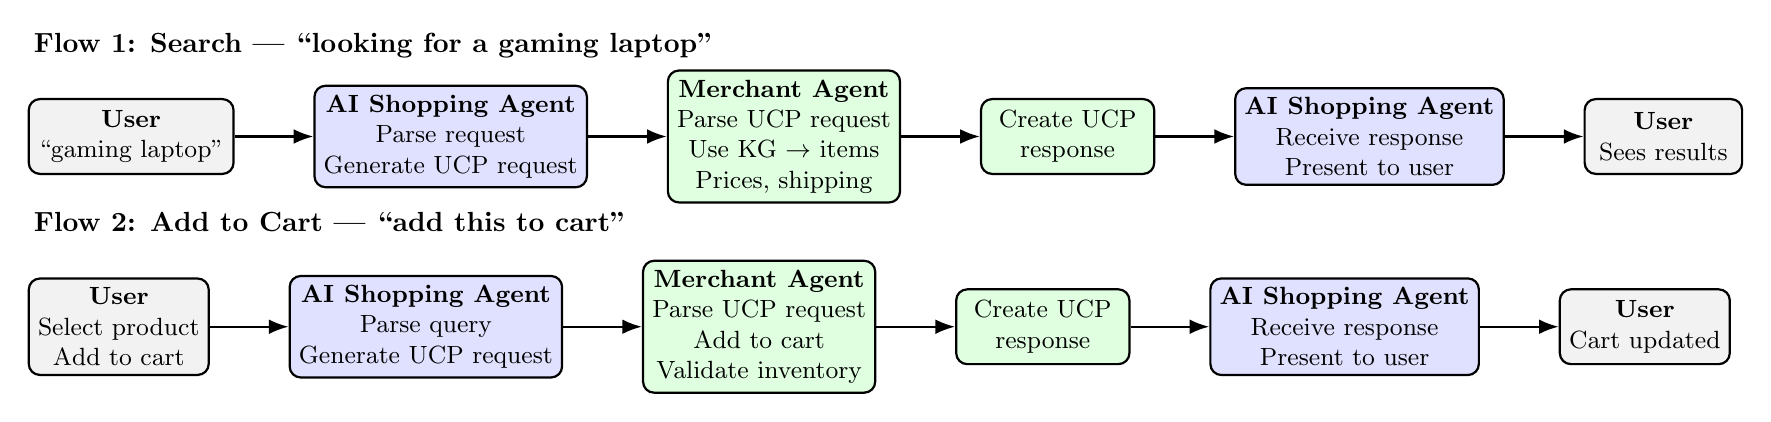
\begin{tikzpicture}[
    box/.style={
        rectangle,
        draw,
        thick,
        rounded corners=4pt,
        align=center,
        minimum height=0.95cm,
        font=\small
    },
    arrow/.style={
        -{Latex[length=2.5mm]},
        thick,
        >=latex
    },
    title/.style={font=\normalsize\bfseries, anchor=west, inner sep=2pt},
    node distance=0.55cm and 0.7cm
]

\def\colA{2cm}
\def\colB{2.5cm}
\def\colC{2.6cm}
\def\colD{2.2cm}
\def\colE{2.2cm}
\def\colF{2cm}
\def\colGap{1cm}

%% ===== FLOW 1: SEARCH =====
\node[title] (f1title) at (0,0)
  {\textbf{Flow 1: Search} --- ``looking for a gaming laptop''};

\node[box, fill=gray!10, below=0.9cm of f1title.north west, anchor=north west,
      minimum width=\colA] (u1) {
  \textbf{User}\\``gaming laptop''};

\node[box, fill=blue!12, right=\colGap of u1.east, anchor=west,
      minimum width=\colB] (ai1a) {
  \textbf{AI Shopping Agent}\\Parse request\\Generate UCP request};

\node[box, fill=green!12, right=\colGap of ai1a.east, anchor=west,
      minimum width=\colC] (ma1a) {
  \textbf{Merchant Agent}\\Parse UCP request\\Use KG $\to$ items\\Prices, shipping};

\node[box, fill=green!12, right=\colGap of ma1a.east, anchor=west,
      minimum width=\colD] (ma1b) {Create UCP\\response};

\node[box, fill=blue!12, right=\colGap of ma1b.east, anchor=west,
      minimum width=\colE] (ai1b) {
  \textbf{AI Shopping Agent}\\Receive response\\Present to user};

\node[box, fill=gray!10, right=\colGap of ai1b.east, anchor=west,
      minimum width=\colF] (u1out) {\textbf{User}\\Sees results};

\draw[arrow] (u1) -- (ai1a);
\draw[arrow] (ai1a) -- (ma1a);
\draw[arrow] (ma1a) -- (ma1b);
\draw[arrow] (ma1b) -- (ai1b);
\draw[arrow] (ai1b) -- (u1out);

%% ===== FLOW 2: ADD TO CART =====
\node[title, anchor=west] (f2title)
  at ([yshift=-0.6cm]f1title.west |- u1.south)
  {\textbf{Flow 2: Add to Cart} --- ``add this to cart''};

\node[box, fill=gray!10, below=0.9cm of f2title.north west, anchor=north west,
      minimum width=\colA] (u2) {
  \textbf{User}\\Select product\\Add to cart};

\node[box, fill=blue!12, right=\colGap of u2.east, anchor=west,
      minimum width=\colB] (ai2a) {
  \textbf{AI Shopping Agent}\\Parse query\\Generate UCP request};

\node[box, fill=green!12, right=\colGap of ai2a.east, anchor=west,
      minimum width=\colC] (ma2a) {
  \textbf{Merchant Agent}\\Parse UCP request\\Add to cart\\Validate inventory};

\node[box, fill=green!12, right=\colGap of ma2a.east, anchor=west,
      minimum width=\colD] (ma2b) {Create UCP\\response};

\node[box, fill=blue!12, right=\colGap of ma2b.east, anchor=west,
      minimum width=\colE] (ai2b) {
  \textbf{AI Shopping Agent}\\Receive response\\Present to user};

\node[box, fill=gray!10, right=\colGap of ai2b.east, anchor=west,
      minimum width=\colF] (u2out) {\textbf{User}\\Cart updated};

\draw[arrow] (u2) -- (ai2a);
\draw[arrow] (ai2a) -- (ma2a);
\draw[arrow] (ma2a) -- (ma2b);
\draw[arrow] (ma2b) -- (ai2b);
\draw[arrow] (ai2b) -- (u2out);

\end{tikzpicture}%
}
\caption{MACS interaction flows. The AI shopping agent handles natural-language
  interaction and protocol generation; the merchant agent enforces hard constraints,
  validates inventory, and returns structured responses. Flow~1 (Search): the user's
  query is parsed, constraint-filtered via the knowledge graph and SQL store, and
  results are returned. Flow~2 (Add to Cart): the merchant agent validates inventory
  before confirming. All constraint enforcement occurs exclusively in the merchant agent.}
\Description{Two interaction flow diagrams. Flow 1 (Search): User to AI Shopping Agent
  (parse request, generate UCP) to Merchant Agent (parse UCP, use KG, prices) to
  Create UCP response to AI Shopping Agent (present to user) to User (sees results).
  Flow 2 (Add to Cart): User to AI Shopping Agent to Merchant Agent (add to cart,
  validate inventory) to Create UCP response to AI Shopping Agent to User (cart updated).}
\label{fig:arch}
\end{figure*}

\begin{figure}[t]
\centering
%% ---------------------------------------------------------------
%% Figure recreated in TikZ (no external PNG dependency).
%% Six stacked "card" nodes with coloured headers, connected by
%% downward arrows, bracketed by User / Merchant-Agent labels.
%%
%% Layout (all coordinates in cm, y increases downward in this
%% design so card tops are at y=0, −1.42, −2.84, …):
%%   card half-width = 3.20  →  total card width 6.40 cm
%%   header height   = 0.42 cm,  body height = 0.70 cm
%%   card height     = 1.12 cm,  inter-card gap = 0.30 cm
%% ---------------------------------------------------------------
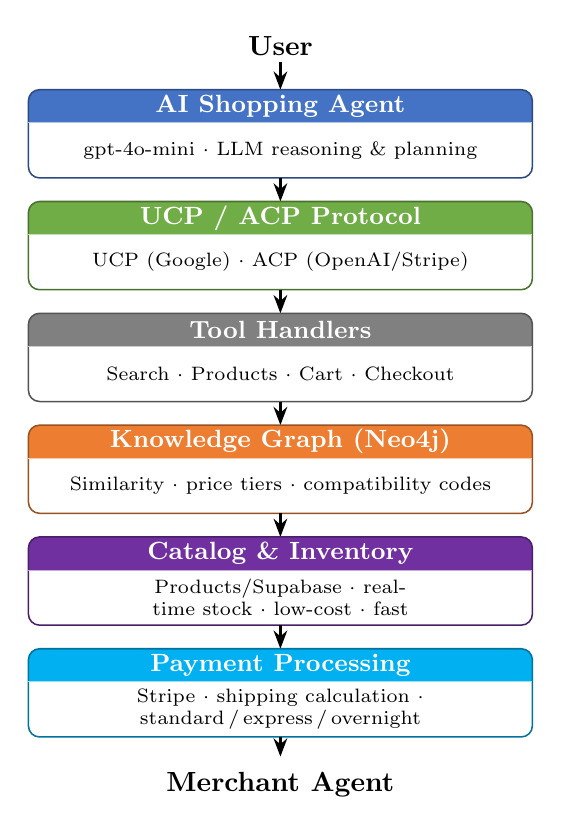
\begin{tikzpicture}[x=1cm, y=1cm]

%% ---- Colour palette (matches original figure) ----
\definecolor{clrAgent}{HTML}{4472C4}     % steel blue  — AI Shopping Agent
\definecolor{clrProtocol}{HTML}{70AD47}  % grass green — UCP/ACP Protocol
\definecolor{clrTools}{HTML}{808080}     % mid-grey    — Tool Handlers
\definecolor{clrKG}{HTML}{ED7D31}        % warm orange — Knowledge Graph
\definecolor{clrCatalog}{HTML}{7030A0}   % deep violet — Catalog \& Inventory
\definecolor{clrPayment}{HTML}{00B0F0}   % sky blue    — Payment Processing

%% ---- Named coordinates (hardcoded for reliable parsing) ----
%% Each card: top (t), header-bottom (h), body-centre (bc),
%%            header-centre (hc), card-bottom (b).  x = ±3.20.

% Card 1 — AI Shopping Agent  (top y = 0.00)
\coordinate (Atl) at (-3.20, 0.00); \coordinate (Atr) at (3.20, 0.00);
\coordinate (Ahl) at (-3.20,-0.42); \coordinate (Ahr) at (3.20,-0.42);
\coordinate (Abl) at (-3.20,-1.12); \coordinate (Abr) at (3.20,-1.12);
\coordinate (Ahc) at (0,-0.21);     \coordinate (Abc) at (0,-0.77);

% Card 2 — UCP / ACP Protocol  (top y = −1.42)
\coordinate (Btl) at (-3.20,-1.42); \coordinate (Btr) at (3.20,-1.42);
\coordinate (Bhl) at (-3.20,-1.84); \coordinate (Bhr) at (3.20,-1.84);
\coordinate (Bbl) at (-3.20,-2.54); \coordinate (Bbr) at (3.20,-2.54);
\coordinate (Bhc) at (0,-1.63);     \coordinate (Bbc) at (0,-2.19);

% Card 3 — Tool Handlers  (top y = −2.84)
\coordinate (Ctl) at (-3.20,-2.84); \coordinate (Ctr) at (3.20,-2.84);
\coordinate (Chl) at (-3.20,-3.26); \coordinate (Chr) at (3.20,-3.26);
\coordinate (Cbl) at (-3.20,-3.96); \coordinate (Cbr) at (3.20,-3.96);
\coordinate (Chc) at (0,-3.05);     \coordinate (Cbc) at (0,-3.61);

% Card 4 — Knowledge Graph  (top y = −4.26)
\coordinate (Dtl) at (-3.20,-4.26); \coordinate (Dtr) at (3.20,-4.26);
\coordinate (Dhl) at (-3.20,-4.68); \coordinate (Dhr) at (3.20,-4.68);
\coordinate (Dbl) at (-3.20,-5.38); \coordinate (Dbr) at (3.20,-5.38);
\coordinate (Dhc) at (0,-4.47);     \coordinate (Dbc) at (0,-5.03);

% Card 5 — Catalog \& Inventory  (top y = −5.68)
\coordinate (Etl) at (-3.20,-5.68); \coordinate (Etr) at (3.20,-5.68);
\coordinate (Ehl) at (-3.20,-6.10); \coordinate (Ehr) at (3.20,-6.10);
\coordinate (Ebl) at (-3.20,-6.80); \coordinate (Ebr) at (3.20,-6.80);
\coordinate (Ehc) at (0,-5.89);     \coordinate (Ebc) at (0,-6.45);

% Card 6 — Payment Processing  (top y = −7.10)
\coordinate (Ftl) at (-3.20,-7.10); \coordinate (Ftr) at (3.20,-7.10);
\coordinate (Fhl) at (-3.20,-7.52); \coordinate (Fhr) at (3.20,-7.52);
\coordinate (Fbl) at (-3.20,-8.22); \coordinate (Fbr) at (3.20,-8.22);
\coordinate (Fhc) at (0,-7.31);     \coordinate (Fbc) at (0,-7.87);

% ============================================================
% USER  (above the stack)
% ============================================================
\node[font=\normalsize\bfseries] at (0, 0.55) {User};
\draw[-Stealth, thick] (0, 0.35) -- (0, 0.00);

% ============================================================
% Cards — drawn with scope+clip so that:
%   • header fill is clipped to the outer rounded rect
%     → top corners are naturally rounded, bottom boundary sharp
%   • body fill is similarly clipped
%     → bottom corners rounded, top boundary sharp
%   • outer border drawn last (rounded corners, coloured)
%   • separator line at the header/body boundary
% ============================================================

% ---- CARD 1 — AI Shopping Agent  (blue) ----
\begin{scope}
  \clip[rounded corners=4pt] (Atl) rectangle (Abr);
  \fill[clrAgent] (Atl) rectangle (Ahr);
  \fill[white]    (Ahl) rectangle (Abr);
\end{scope}
\draw[clrAgent!65!black, rounded corners=4pt, line width=0.55pt]
  (Atl) rectangle (Abr);
\draw[clrAgent!40, line width=0.3pt] (Ahl) -- (Ahr);
\node[text=white, font=\small\bfseries, anchor=center] at (Ahc)
  {AI Shopping Agent};
\node[font=\scriptsize, text width=5.9cm, align=center, anchor=center] at (Abc)
  {gpt-4o-mini $\cdot$ LLM reasoning \& planning};
\draw[-Stealth, thick] (0,-1.12) -- (0,-1.42);

% ---- CARD 2 — UCP / ACP Protocol  (green) ----
\begin{scope}
  \clip[rounded corners=4pt] (Btl) rectangle (Bbr);
  \fill[clrProtocol] (Btl) rectangle (Bhr);
  \fill[white]       (Bhl) rectangle (Bbr);
\end{scope}
\draw[clrProtocol!65!black, rounded corners=4pt, line width=0.55pt]
  (Btl) rectangle (Bbr);
\draw[clrProtocol!40, line width=0.3pt] (Bhl) -- (Bhr);
\node[text=white, font=\small\bfseries, anchor=center] at (Bhc)
  {UCP / ACP Protocol};
\node[font=\scriptsize, text width=5.9cm, align=center, anchor=center] at (Bbc)
  {UCP (Google) $\cdot$ ACP (OpenAI/Stripe)};
\draw[-Stealth, thick] (0,-2.54) -- (0,-2.84);

% ---- CARD 3 — Tool Handlers  (grey) ----
\begin{scope}
  \clip[rounded corners=4pt] (Ctl) rectangle (Cbr);
  \fill[clrTools] (Ctl) rectangle (Chr);
  \fill[white]    (Chl) rectangle (Cbr);
\end{scope}
\draw[clrTools!65!black, rounded corners=4pt, line width=0.55pt]
  (Ctl) rectangle (Cbr);
\draw[clrTools!40, line width=0.3pt] (Chl) -- (Chr);
\node[text=white, font=\small\bfseries, anchor=center] at (Chc)
  {Tool Handlers};
\node[font=\scriptsize, text width=5.9cm, align=center, anchor=center] at (Cbc)
  {Search $\cdot$ Products $\cdot$ Cart $\cdot$ Checkout};
\draw[-Stealth, thick] (0,-3.96) -- (0,-4.26);

% ---- CARD 4 — Knowledge Graph (Neo4j)  (orange) ----
\begin{scope}
  \clip[rounded corners=4pt] (Dtl) rectangle (Dbr);
  \fill[clrKG] (Dtl) rectangle (Dhr);
  \fill[white] (Dhl) rectangle (Dbr);
\end{scope}
\draw[clrKG!65!black, rounded corners=4pt, line width=0.55pt]
  (Dtl) rectangle (Dbr);
\draw[clrKG!40, line width=0.3pt] (Dhl) -- (Dhr);
\node[text=white, font=\small\bfseries, anchor=center] at (Dhc)
  {Knowledge Graph (Neo4j)};
\node[font=\scriptsize, text width=5.9cm, align=center, anchor=center] at (Dbc)
  {Similarity $\cdot$ price tiers $\cdot$ compatibility codes};
\draw[-Stealth, thick] (0,-5.38) -- (0,-5.68);

% ---- CARD 5 — Catalog \& Inventory  (violet) ----
\begin{scope}
  \clip[rounded corners=4pt] (Etl) rectangle (Ebr);
  \fill[clrCatalog] (Etl) rectangle (Ehr);
  \fill[white]      (Ehl) rectangle (Ebr);
\end{scope}
\draw[clrCatalog!65!black, rounded corners=4pt, line width=0.55pt]
  (Etl) rectangle (Ebr);
\draw[clrCatalog!40, line width=0.3pt] (Ehl) -- (Ehr);
\node[text=white, font=\small\bfseries, anchor=center] at (Ehc)
  {Catalog \& Inventory};
\node[font=\scriptsize, text width=5.9cm, align=center, anchor=center] at (Ebc)
  {Products/Supabase $\cdot$ real-time stock $\cdot$ low-cost $\cdot$ fast};
\draw[-Stealth, thick] (0,-6.80) -- (0,-7.10);

% ---- CARD 6 — Payment Processing  (sky blue) ----
\begin{scope}
  \clip[rounded corners=4pt] (Ftl) rectangle (Fbr);
  \fill[clrPayment] (Ftl) rectangle (Fhr);
  \fill[white]      (Fhl) rectangle (Fbr);
\end{scope}
\draw[clrPayment!65!black, rounded corners=4pt, line width=0.55pt]
  (Ftl) rectangle (Fbr);
\draw[clrPayment!40, line width=0.3pt] (Fhl) -- (Fhr);
\node[text=white, font=\small\bfseries, anchor=center] at (Fhc)
  {Payment Processing};
\node[font=\scriptsize, text width=5.9cm, align=center, anchor=center] at (Fbc)
  {Stripe $\cdot$ shipping calculation $\cdot$ standard\,/\,express\,/\,overnight};

% ============================================================
% MERCHANT AGENT  (below the stack)
% ============================================================
\draw[-Stealth, thick] (0,-8.22) -- (0,-8.47);
\node[font=\normalsize\bfseries] at (0,-8.82) {Merchant Agent};

\end{tikzpicture}
\caption{Conceptual overview of the MACS merchant-agent framework showing the
  separation between the AI shopping agent (natural-language interaction) and
  the merchant agent (deterministic constraint enforcement and catalog access).}
\Description{Conceptual diagram showing the MACS system with the shopping agent
  and merchant agent layers and their interaction boundary.}
\label{fig:concept}
\end{figure}

\subsection{Protocol and Data Layer}

MACS exposes three protocol families from a single canonical backend, so
adding a new protocol requires only a request adapter and response formatter.
\textbf{MCP}~\cite{Anthropic2024MCP} provides four typed tool calls
(\texttt{search\_products}, \texttt{get\_product}, \texttt{add\_to\_cart},
\texttt{checkout}) with observable response envelopes.
\textbf{UCP}~\cite{UCPGoogle2026} follows Google's schema for Gemini-based agents.
\textbf{ACP}~\cite{ACPOpenAI2025} adds a checkout session lifecycle and webhooks;
a config variable selects UCP vs.\ ACP at deploy time.

\subsection{Data Layer}

Three data stores serve distinct roles.

\textbf{Relational product store} holds the authoritative product catalog
(21,000+ items; 1,490+ laptops with 12 structured spec fields per product:
CPU, RAM, GPU, storage type, display size, battery life, weight, OS, price,
brand, review count, and rating).
All correctness-critical operations---constraint filtering, brand exclusion,
progressive relaxation---execute as SQL queries against this store.

\textbf{Knowledge graph} encodes product relationships across
2,400 nodes and 8,500 edges in four relationship types:
\textsc{Similar\_To} (same use-case substitutes at similar price),
\textsc{Compatible\_With} (accessory compatibility),
\textsc{Manufactured\_By} (brand graph), and
\textsc{Use\_Case} (product-to-use-case mapping).
Complex intent queries (``show me similar items,'' ``find a compatible
accessory'') are resolved via Cypher traversal in $\sim$17~ms with no LLM call.
The graph degrades gracefully to SQL-based search when unavailable,
ensuring no hard dependency on the graph layer.

\textbf{Cache and session layer} caches search results, product summaries,
price data, and LLM-generated narratives using per-entry Time-To-Live (TTL)
expirations (30~s--10~min depending on data freshness requirements).
This achieves $\sim$12$\times$ latency reduction on cache hits
(36~ms vs.\ 446~ms cold read, measured over $n = 10$ runs).

%% --------------------------------------------------------------------------
%% Algorithmic subsections — query rewriting and criteria extraction run in
%% the shopping agent (Section~\ref{sec:shopping-agent}); the merchant agent
%% receives the extracted slot dictionary and executes the steps below.
%% --------------------------------------------------------------------------

\subsection{Hard Constraint Filtering}

Extracted slot values map directly to SQL \texttt{WHERE} clauses.
Brand exclusions are enforced both at the SQL level and in a post-retrieval
filter that checks the product title---necessary for products in which the
database brand field stores condition (``New'', ``Recertified'') rather than
the manufacturer name.

\subsection{Progressive Relaxation}

When hard constraints produce fewer than three results, the system
applies a sequence of relaxation steps ordered by constraint importance.
At each step, the least-critical optional specification constraint is dropped
first, while correctness-critical filters---price ceiling and brand
exclusions---are never relaxed.
The user always sees real, purchasable products; the system never returns an
empty result set or fabricated alternatives.
When relaxation occurs, the response explicitly discloses which constraints
were loosened, so the user is not misled about what was actually enforced.

\subsection{Best-Value Scoring}

The best-value pick uses a weighted scoring function tuned to the detected
use case:

\begin{equation}
\text{score}(p) = w_{\text{price}} \cdot r_p +
                  w_{\text{rating}} \cdot \hat{r} +
                  w_{\text{vol}} \cdot \log(n+1) +
                  w_{\text{spec}} \cdot \phi(p)
\end{equation}

where $p$ denotes a product; $r_p \in [0,1]$ is the normalized price score
computed as $1 - ({\rm price}_p - {\rm price}_{\min}) / ({\rm price}_{\max} -
{\rm price}_{\min})$, so lower-priced products receive higher scores within
the retrieved set; $\hat{r}$ is the star rating; $n$ is review count; and
$\phi(p) \in [0,1]$ is a use-case spec score---a weighted sum of
specification relevance indicators (e.g., GPU tier weight for gaming queries,
battery-life weight for travel queries, price-efficiency weight for
student/budget queries). $\phi(p)$ is not a learned similarity score; it is
a deterministic weighted sum over structured spec fields extracted from the catalog.

%% ==========================================================================
\section{Evaluation}
%% ==========================================================================

\subsection{Benchmark Design and Ground Truth Construction}
\label{sec:evaluation}

The evaluation separates \emph{constraint correctness} (enforcing price, brand,
and spec requirements) from \emph{response quality} (helpful, well-explained
recommendations). Hard constraints are evaluated deterministically via SQL
verification. For response quality, we use G-Eval~\cite{Liu2023GEval}---an
LLM-as-judge evaluation framework that scores free-text responses against a
rubric without requiring gold-standard reference answers---restricted to
quality assessment to avoid circularity with the constraint-checking component.

\paragraph{Deterministic ground truth (hard constraints).}
For each benchmark query, expected filter values and exclusions
are derived by executing the constraints directly against the relational
product store as SQL predicates
(e.g., {\small\texttt{price <= 1000 AND brand NOT ILIKE '\%HP\%'}}).
This ground truth is independent of any LLM: violations are verifiable,
objective failures. The approach eliminates the circularity problem of using
one LLM to generate reference answers and another to judge whether the
system matches them.

\paragraph{LLM-as-judge quality scoring.}
For response narrative quality, G-Eval is applied with a
custom rubric evaluating engagement (0--4), tone calibration (0--3), and
factual accuracy/coherence (0--3), normalized to $[0,1]$.
The judge is GPT-4o-mini at temperature 0 for reproducibility.
It evaluates whether explanations are factually grounded in the returned
products---not whether they resemble a reference answer.
Calibration examples anchor scores at 0.0, 0.5, and 1.0 to reduce judge
variance.

\paragraph{Composite scoring formula.}
The final per-query score combines deterministic and quality components:
\begin{equation}
  s = 0.40\,s_{\text{type}} + 0.20\,s_{\text{brand}} + 0.10\,s_{\text{filter}}
    + 0.05\,s_{\text{stock}} + 0.10\,s_{\text{explain}} + 0.15\,s_{\text{quality}}
  \label{eq:geval}
\end{equation}
where $s_{\text{type}} \in \{0,1\}$ is a binary response-type match
(1 if the system produces a recommendation when one is expected, or a
clarifying question when the query is underspecified; 0 otherwise);
$s_{\text{brand}} \in [0,1]$ is the fraction of returned products respecting
all stated brand exclusions;
$s_{\text{filter}} \in [0,1]$ is the fraction of returned products satisfying
price and specification constraints;
$s_{\text{stock}} \in [0,1]$ is the fraction of returned products that are
currently available in inventory (i.e., not marked out-of-stock or
discontinued in the catalog at query time);
$s_{\text{explain}} \in [0,1]$ measures response explainability deterministically
via three equal-weight sub-checks: whether the message contains structured
explanation elements (bullet lists or explanatory connectives such as
\emph{because} or \emph{since}), at least one specific product attribute
(e.g., RAM, battery life, price, or storage), and an explicit disclosure of
applied constraints (e.g., ``under \$X,'' ``at least,'' or ``matching your'');
each sub-check contributes equally so
$s_{\text{explain}} = \text{checks\_passed} / 3$;
and $s_{\text{quality}} \in [0,1]$ is the G-Eval narrative quality score.
Weights for components inapplicable to a given query (e.g., $s_{\text{brand}}$
when no brand exclusion is present, or $s_{\text{explain}}$ for
clarification-only responses) are redistributed to $s_{\text{quality}}$,
raising its effective weight to 45--60\%.
This redistribution means text-only baselines (GPT, Gemini) are evaluated
on $s_{\text{type}}$ and $s_{\text{quality}}$ in their composite scores;
brand compliance is additionally checked via a negation-window regex over
free-text responses (reported separately in Table~\ref{tab:results160},
not folded into the composite), and filter compliance remains N/A as
price verification from free text is unreliable.

\paragraph{Query construction.}
Queries were authored by the research team to cover five user intent classes:
direct purchase (e.g., ``gaming laptop under \$1{,}000 with at least 16\,GB RAM,
no HP''), multi-constraint filtering, vague preference (e.g., ``I need something
for school''), service inquiry (e.g., ``What is your return policy on
refurbished laptops?''), and product comparison.
These five classes were selected to stress-test the core design constraint:
a merchant-deployed system must handle the full spectrum from maximally vague
(preference elicitation required before any retrieval) to maximally precise
(simultaneous enforcement of multiple hard constraints).
Each query is assigned a buyer persona (student, professional, gamer, or
traveler) drawn from archetypes observed in online product-review communities;
these four personas generate meaningfully distinct constraint profiles
(budget sensitivity, portability requirements, performance thresholds, and
brand loyalty patterns) while remaining representative of the shopping agent
use cases studied in ShoppingBench~\cite{Wang2025ShoppingBench}.
Each query is classified as \emph{specified}---containing $\geq$1 extractable
hard constraint (brand exclusion, price ceiling, or minimum specification)---or
\emph{underspecified}---expressing intent without measurable constraints.

\paragraph{Benchmark scale.}
Two nested sets are used.
The \emph{shared 140-query benchmark} (85 specified / 55 underspecified) supports
a three-way comparison across MACS, \GPTCatalog{}, and \GeminiCatalog{}.
The \emph{expanded 225-query benchmark} (138 specified / 87 underspecified)
covers 40 query groups including catalog exploration, follow-up service questions,
post-recommendation refinements, and orchestrator routing; this set is evaluated
on MACS only due to the cost of running all baselines at this scale.
Pass threshold: score $\geq 0.5$.

\paragraph{Stochastic robustness.}
The G-Eval judge introduces $\approx$0.02--0.03 score variance between
identical runs at temperature~0.
PASS@$k$~\cite{Chen2021Codex}---the fraction of $k$ independent evaluation
runs that pass---provides a robustness measure for this variance.
We evaluate PASS@5 on the 225-query benchmark using a pre-fix code snapshot:
MACS achieves a macro PASS@5 of $0.742$, with mean score $0.609 \pm 0.010$ (SD)
across five independent runs (per-run averages: $0.622, 0.614, 0.611, 0.603, 0.596$;
pass rate $74.2\% \pm 4.2$pp). The $\pm 0.010$ SD confirms that single-run
results lie within one SD of the multi-run mean; the same variance bound applies
to the improved result of $0.681$ (Table~\ref{tab:groups}) from the final code
version.

\subsection{Multi-Turn Evaluation Design}
\label{sec:multiturn-eval}

Single-turn evaluations cannot assess the properties that distinguish agentic
systems from stateless LLM calls: constraint persistence, preference updates,
and brand-exclusion reversals across turns.
A 10-scenario multi-turn benchmark is designed covering six
constraint-persistence patterns: constraint accumulation, use-case pivot
(gaming $\to$ video editing), brand-exclusion persistence, vague-to-specific
elicitation, budget overwrite (update, not accumulate), and exclusion reversal
(``HP is fine now''). Scenarios also include a full 5-turn medical-student
purchase flow and a dense multi-constraint first turn. Each scenario contains
3--5 scripted turns.

\paragraph{Scoring.}
The multi-turn score combines a judge score with deterministic constraint checks:
\begin{equation}
  s_{\text{MT}} = 0.55\,s_{\text{constraint}} + 0.45\,s_{\text{judge}}
  \label{eq:multiturn}
\end{equation}
$s_{\text{constraint}}$ is computed from deterministic checks against the
system's final-turn product list: brand exclusions present/absent, budget
ceiling respected. Critically, constraint checks run \emph{before} the judge,
and their results (pass/fail notes) are injected into the judge prompt so
the judge can calibrate without hallucinating failures on silently-enforced
constraints. $s_{\text{judge}}$ is GPT-4o-mini (temperature 0) evaluating
the full conversation transcript on constraint satisfaction (0--4), preference
tracking accuracy (0--3), and response appropriateness (0--3).
Pass threshold: $\geq 0.65$ (raised from 0.50 to eliminate floor effects:
a system with $s_{\text{constraint}}=1.0$ and judge=0 would auto-pass at
threshold 0.50 since $0.55\times 1 + 0.45 \times 0 = 0.55 \geq 0.50$).
\emph{Mean score} reported in tables is the average of $s_{\text{MT}}$
across all $K$ independent runs for each scenario, then averaged across scenarios.
\emph{Macro Pass@K} is the mean over scenarios of the fraction of K runs exceeding
the threshold (i.e., the fraction of runs that pass, averaged over all scenarios).

\paragraph{Fair catalog-bound baselines.}
Before each baseline turn, MACS's search endpoint retrieves the top-10
products, which are injected into the baseline's system prompt. All systems
therefore recommend from an identical live catalog snapshot, isolating
architecture differences from database access gaps.

\subsection{Latency Measurement}

The full request lifecycle is instrumented with phase-level timing logged in
each MCP response envelope. Table~\ref{tab:latency} shows representative
latencies for each phase.

\begin{table}[t]
  \caption{Measured \textbf{median} latencies by pipeline phase ($n = 10$
  runs per phase, direct-call benchmark; median reported, not mean, to
  reduce sensitivity to occasional LLM cold-start outliers). LLM calls
  dominate total latency; knowledge graph traversal and cache hits are
  negligible.}
  \label{tab:latency}
  \small
  \begin{tabular}{@{}lrp{2.5cm}@{}}
    \toprule
    Phase & Median (ms) & Notes \\
    \midrule
    CPU phases (rewrite, filter)  &   $<$1        & Pure Python, no I/O \\
    Domain detection — fast path  &   $<$1        & Keyword dictionary \\
    Domain detection — LLM        & $\sim$1{,}630 & gpt-4o-mini; ambiguous only \\
    Criteria extraction (LLM)     & 1{,}927       & Primary bottleneck \\
    Question generation (LLM)     & 1{,}645       & Preference elicitation \\
    Post-rec intent detection     &   556         & gpt-4o-mini classification \\
    Rec.\ narrative (LLM)         & 2{,}256       & Recommendation explanation \\
    Comparison narrative (LLM)    & 5{,}714       & Longest single phase \\
    Filter refinement (LLM)       & 2{,}187       & gpt-4o-mini refinement \\
    SQL search (cache miss)       &   446         & catalog store round-trip \\
    SQL search (cache hit)        &    36         & cache GET + deserialize \\
    KG re-ranking overlay         &   207         & FAISS + graph + scoring \\
    Total (cache miss, rec.)      & $\sim$4{,}600 & Criteria + SQL + narrative \\
    Total (cache hit, rec.)       & $\sim$2{,}300 & Criteria + cache \\
    \bottomrule
  \end{tabular}
\end{table}

LLM inference accounts for 85--92\% of total latency on cache misses.
The knowledge graph re-ranking overlay (207~ms median) is 11--28$\times$ faster
than equivalent LLM-based narrative generation (2,256--5,714~ms median) and
produces deterministic, auditable results. Structural queries (substitutes,
best value) should route through the graph, not a prompt.

The cache layer reduces effective latency $\sim$12$\times$ on repeated queries
(446~ms cold vs.\ 36~ms cached; popular product categories, frequently compared
spec configurations).

\subsection{Single-Turn Quality Results}

\GPTCatalog{} and \GeminiCatalog{} each receive MACS's live catalog per
query (catalog grounding = 1.0), so all three systems recommend from identical
product pools. MACS brand and filter scores are evaluated deterministically via SQL.
For text-only baselines, brand compliance is approximated by a
negation-window regex over free-text responses (6 exclusion queries);
filter compliance cannot be verified from free text and remains N/A.
All systems use the same token budget and are prohibited from web search.

\begin{table}[t]
  \caption{Three-way single-turn comparison ($n = 140$ queries, pass
  threshold $\geq 0.5$; April 2026 clean run, real quality scoring).
  MACS Brand/Filter: deterministic SQL-layer compliance.
  Baseline Brand$^\dagger$: regex negation-window check on free-text responses
  (6 exclusion queries; 1 Gemini violation on Q26 ``no HP, no Acer'').
  Filter N/A: cannot verify price compliance from free text.
  Quality: LLM-judge narrative score (GPT-4o-mini, temperature~0).}
  \label{tab:results160}
  \begin{tabular}{lrrrrr}
    \toprule
    System & Avg $\uparrow$ & Pass\% $\uparrow$ & Brand $\uparrow$ & Filter $\uparrow$ & Quality $\uparrow$ \\
    \midrule
    MACS             & \textbf{0.681} & \textbf{87.1\%} & \textbf{1.000} & \textbf{0.970} & 0.394 \\
    \GeminiCatalog{} & 0.662          & 68.6\%          & 0.833$^\dagger$ & N/A   & \textbf{0.427} \\
    \GPTCatalog{}    & 0.639          & 72.1\%          & 1.000$^\dagger$ & N/A   & 0.392 \\
    \bottomrule
  \end{tabular}
\end{table}

\begin{table}[t]
  \caption{Combined single-turn (ST, 140 queries, threshold $\geq 0.5$) and
  multi-turn (MT, 10 scenarios, K=5 runs, threshold $\geq 0.65$) results.
  MT scoring: $0.55\times$constraint (deterministic) $+$ $0.45\times$judge
  (GPT-4o-mini, temp.~0). All systems catalog-bound; same token budget; no web
  search. Pass@5 = macro fraction of K runs passing threshold.
  Drift: fraction of run-scenario pairs with a constraint violation.}
  \label{tab:combined}
  \footnotesize\setlength{\tabcolsep}{4pt}%
  \begin{tabular}{@{}lrrrrr@{}}
    \toprule
    & \multicolumn{2}{c}{Single-Turn} & \multicolumn{3}{c}{Multi-Turn} \\
    \cmidrule(lr){2-3}\cmidrule(lr){4-6}
    System & ST Avg & ST Pass\% & MT Avg$\pm$SD & MT Pass@5 & Drift \\
    \midrule
    MACS             & \textbf{0.681} & \textbf{87.1\%} & 0.739$\pm$0.110 & \textbf{60\%} & \textbf{0.000} \\
    \GPTCatalog{}    & 0.639          & 72.1\%          & \textbf{0.747}$\pm$0.088 & 54\%          & \textbf{0.000} \\
    \GeminiCatalog{} & 0.662          & 68.6\%          & 0.727$\pm$0.112 & 52\%          & \textbf{0.000} \\
    \bottomrule
  \end{tabular}
\end{table}

MACS leads all systems on single-turn pass rate at 87.1\%
(Table~\ref{tab:results160},~\ref{tab:combined}), with perfect brand and
near-perfect filter compliance (1.000/0.970). \GPTCatalog{} achieves 72.1\% and
\GeminiCatalog{} 68.6\%; the gap reflects MACS's SQL-enforced constraint pipeline,
which text-only systems cannot replicate structurally.
Remaining MACS failures are catalog-level: absent inventory, marketplace risk,
and multi-category budgets.

\emph{Scope note}: all evaluations use a consumer-electronics catalog
(laptops and accessories). Generalization to other product domains is not
claimed and represents a direction for future work.

\subsection{Expanded 225-Query Benchmark}
\label{sec:expanded}

The 43-query benchmark assesses core functionality but is too small to support
per-group pass-rate comparisons without overfitting concerns.
To address this, the benchmark is expanded to 225 queries spanning 40 distinct
interaction groups, including catalog exploration, service follow-up questions
(return policy, shipping, warranty), post-recommendation refinements, and
orchestrator routing. Table~\ref{tab:groups} summarizes performance on the
eight groups where MACS most clearly succeeds or struggles.

\begin{table}[t]
  \caption{Per-group single-turn results on the expanded 225-query benchmark
  (MACS only; pass threshold: $\geq 0.5$). All queries are evaluated
  independently (no prior session context).}
  \label{tab:groups}
  \begin{tabular}{lrrr}
    \toprule
    Group & $N$ & Avg $\uparrow$ & Pass\% $\uparrow$ \\
    \midrule
    \multicolumn{4}{l}{\textit{Strong groups}} \\
    Multi-intent rigidity      &  5 & 0.775 & 100.0\% \\
    One-liner purchase intent  &  6 & 0.833 & 100.0\% \\
    Refinement                 &  3 & 0.756 & 100.0\% \\
    Follow-up service QA       &  4 & 0.810 & 100.0\% \\
    Multi-constraint           & 17 & 0.791 &  94.1\% \\
    Post-rec refinement        &  7 & 0.738 &  85.7\% \\
    \midrule
    \multicolumn{4}{l}{\textit{Weak groups}} \\
    Context-free comparison    &  6 & 0.393 &   0.0\% \\
    Orchestrator routing       & 12 & 0.502 &  33.3\% \\
    Preference discovery       &  8 & 0.473 &  25.0\% \\
    \midrule
    \textbf{All (225 queries)} & 225 & \textbf{0.681} & \textbf{85.3\%} \\
    \bottomrule
  \end{tabular}
\end{table}

Across 225 queries, MACS achieves avg.\ 0.681 (pass rate 85.3\%), up from
0.604/74.2\%. Key gains from targeted fixes: follow-up service QA
(0\%$\to$100\%); catalog exploration (50\%$\to$75\%); orchestrator routing
(25\%$\to$33\%); post-rec refinement (43\%$\to$86\%); gaming-specific
(25\%$\to$100\%). The multi-constraint group (17 queries) achieves 94.1\%
pass rate, confirming that the SQL pipeline enforces four simultaneous
constraints deterministically.

Weak groups are structural failures: the context-free comparison (0\%) and
orchestrator routing (33\%) groups contain queries referencing prior results
or session actions (compare, add-to-cart) absent in a fresh session---these
are inherently multi-turn and require pre-populated session context the
single-turn benchmark cannot provide.

\paragraph{Failure mode analysis.}
The three persistent weak areas reflect identifiable system limitations rather than
random noise.
\emph{Context-free comparison} (0.0\%): queries such as ``compare those two'' or
``which of these is better'' arrive without a prior recommendation in session state;
single-turn evaluation structurally cannot provide one.
\emph{Orchestrator routing} (33.3\%): multi-intent requests that mix recommendation,
comparison, and cart actions in a single turn exceed the single-dispatch routing
architecture; routing accuracy requires compound-sentence decomposition not yet
implemented.
\emph{Long session} (S9, 0\% Pass@5, multi-turn): the 10-turn session history window
in the session manager truncates constraints stated before turn~11; preference state
accumulated in early turns is partially lost.
Fixing long-session failure modes requires persistent preference
logs beyond the turn window---a direction for future work.

\subsection{Multi-Turn Constraint Results}
\label{sec:multiturn-results}

Table~\ref{tab:combined} reports combined single-turn and multi-turn results
(K=5 runs, threshold $\geq 0.65$). MACS leads all systems on macro Pass@5
(\textbf{60\%} vs.\ 54\% \GPTCatalog{} vs.\ 52\% \GeminiCatalog{}).
Mean score is 0.739 for MACS vs.\ 0.747 GPT vs.\ 0.727 Gemini---within one SD,
indicating the systems are statistically tied on mean quality while MACS
leads on the binary Pass@5 metric.
MACS uniquely achieves 100\% Pass@5 on Exclusion Reversal---the
scenario requiring mid-session constraint state updates---where
\GPTCatalog{} scores only 20\% and \GeminiCatalog{} scores 0\%
(Table~\ref{tab:multiturn_cat}). MACS also leads on Brand Exclusion
persistence (80\% vs.\ 40\%/0\%), Dense Constraint (100\% vs.\ 80\%/80\%),
and Budget Overwrite (100\% vs.\ 80\%/100\%).

MACS enforces constraints as SQL-level predicates persisted in the session
store, so they cannot be dropped by LLM inference across turns.
The session-persistent exclusion-un-exclusion pathway achieves Pass@5=100\%
(vs.\ 20\% for \GPTCatalog{} and 0\% for \GeminiCatalog{}), a
gap attributable to MACS's explicit \texttt{\_detect\_allowed\_brands()}
pathway and deterministic spec-constraint accumulation across turns.
\GPTCatalog{} outperforms on long-session (100\% vs.\ 0\%) and
clarification scenarios (100\% each), where a well-structured single-turn
LLM call suffices without accumulated constraint state. All three systems
achieve zero constraint drift across all 50 run-scenario pairs.

\begin{table}[t]
  \caption{Multi-turn category breakdown (K=5 runs; avg score / Pass@5;
  \checkmark~= Pass@5~$\geq 60$\%). Categories map 1:1 to the 10 scenarios.}
  \label{tab:multiturn_cat}
  \footnotesize\setlength{\tabcolsep}{4pt}%
  \begin{tabular}{@{}lccc@{}}
    \toprule
    Category & MACS & \GPTCatalog{} & \GeminiCatalog{} \\
    \midrule
    Brand Exclusion       & \checkmark 0.721 / 80\%  & 0.757 / 40\%             & 0.640 / 0\%   \\
    Budget Overwrite      & \checkmark 0.865 / 100\% & \checkmark 0.757 / 80\%  & \checkmark 0.838 / 100\% \\
    Budget Refinement     & \checkmark 0.802 / 80\%  & \checkmark 0.802 / 80\%  & \checkmark 0.838 / 100\% \\
    Clarification         & \checkmark 0.757 / 100\% & \checkmark 0.856 / 100\% & \checkmark 0.802 / 100\% \\
    Comparison            & 0.622 / 0\%              & 0.640 / 0\%              & 0.604 / 0\%   \\
    Constraint Persist.   & \checkmark 0.784 / 40\%  & 0.748 / 40\%             & 0.685 / 40\%  \\
    Dense Constraint      & \checkmark 0.694 / 100\% & \checkmark 0.802 / 80\%  & \checkmark 0.874 / 80\%  \\
    Exclusion Reversal    & \checkmark 0.946 / 100\% & 0.622 / 20\%             & 0.586 / 0\%   \\
    Intent Pivot          & 0.613 / 0\%              & 0.631 / 0\%              & 0.613 / 0\%   \\
    Long Session          & 0.586 / 0\%              & \checkmark 0.856 / 100\% & \checkmark 0.793 / 100\% \\
    \midrule
    Overall               & \textbf{0.739 / 60\%}    & 0.747 / 54\%             & 0.727 / 52\%  \\
    \bottomrule
  \end{tabular}
\end{table}

\begin{table}[t]
  \centering
  \small
  \caption{Pass@5 per scenario (K=5, threshold=0.65). \checkmark{} marks a unique MACS win
           (all others score $<$60\%). Bold = highest pass rate per row.}
  \label{tab:multiturn_scenario}
  \begin{tabular}{lccc}
    \toprule
    \textbf{Scenario} & \textbf{MACS} & \textbf{GPT+Cat.} & \textbf{Gemini+Cat.} \\
    \midrule
    S1: Constraint Accumulation   & 40\%                      & \textbf{40\%}  & \textbf{40\%} \\
    S2: Mind-Change Pivot         & 0\%                       & 0\%            & 0\%           \\
    S3: Brand Excl.\ Persistence  & \checkmark \textbf{80\%}  & 40\%           & 0\%           \\
    S4: Vague $\to$ Specific      & \checkmark \textbf{100\%} & \textbf{100\%} & \textbf{100\%}\\
    S5: Comparison + Follow-up    & 0\%                       & 0\%            & 0\%           \\
    S6: Price Refinement          & 80\%                      & 80\%           & \textbf{100\%}\\
    S7: Budget Overwrite          & \checkmark \textbf{100\%} & 80\%           & \textbf{100\%}\\
    S8: Exclusion Reversal (HP)   & \checkmark \textbf{100\%} & 20\%           & 0\%           \\
    S9: Long Session (5-turn)     & 0\%                       & \textbf{100\%} & \textbf{100\%}\\
    S10: Dense Constraint         & \checkmark \textbf{100\%} & 80\%           & 80\%          \\
    \midrule
    Overall (macro Pass@5)        & \textbf{60\%}             & 54\%           & 52\%          \\
    \bottomrule
  \end{tabular}
\end{table}

Table~\ref{tab:multiturn_cat} groups results by constraint category.
MACS uniquely dominates exclusion reversal (100\% Pass@5 vs.\ 20\% GPT / 0\%
Gemini) and brand exclusion persistence (80\% vs.\ 40\%/0\%)---both require
mid-conversation state updates via session-persisted slot dictionaries.
MACS also achieves 100\% on dense constraint (vs.\ 80\%/80\%), driven by the
deterministic spec-accumulation pathway that ensures incremental constraints
("also needs at least 16GB RAM") are always applied to subsequent searches.
\GPTCatalog{} leads on long session (100\% vs.\ 0\%), where a single
well-structured LLM context suffices without persistent state.
Intent pivot and comparison score 0\% across all three systems, confirming
these are fundamentally multi-turn failure modes rather than system-specific weaknesses.

\subsection{Trust \& Safety Evaluation}
\label{sec:trust}

Standard quality metrics measure \emph{what} a system recommends; they do not
measure whether it behaves safely under adversarial or underspecified inputs.
Three Trust \& Safety pillars are evaluated, each measured deterministically.
All three assess whether the system provides the \emph{guarantees}
central to the design: enforcing constraints when possible, persisting them
across turns, and disclosing honestly when they cannot be met.

\paragraph{Inventory integrity (\emph{Grounding}).}
\emph{Grounding} is the fraction of returned product identifiers that exist in
the catalog at the stated price. A score of 1.0 means every recommended product
is real and purchasable; a stateless LLM generating free text would score
$\approx$0.00. MACS, \GPTCatalog{}, and \GeminiCatalog{} all score 1.000
because all three use MACS's catalog layer exclusively.

\paragraph{Preference fidelity (\emph{Drift}).}
\emph{Constraint drift} is measured as: drift rate = violations / applicable
(turn, constraint) pairs across all runs and scenarios. For each multi-turn
scenario, active constraints (brand exclusions, budget ceilings) are annotated
per turn; a violation is recorded any time a returned product breaks a still-active
constraint. A drift rate of 0.000 means zero constraint violations across all
$K \times |\text{scenarios}|$ run-scenario pairs---stronger than checking only
the final turn. MACS scores 0.000 (zero violations across all 50 run-scenario pairs).
\GPTCatalog{} and \GeminiCatalog{} also achieve 0.000 in the April 2026
run, indicating that catalog-bound baselines---when given the identical
product pool---reliably avoid out-of-constraint recommendations even
without session persistence, as long as the constraint is still in the
active context window.

\paragraph{Honest scoping (\emph{Disclosure}).}
\emph{Disclosure} measures whether the system honestly communicates when a
user's constraints cannot be fully satisfied. Eight \emph{catalog-impossible}
queries are constructed---requests whose stated constraints no product can
meet (e.g., ``gaming laptop with RTX~4090, budget \$150'').
Scoring: 1.0 for explicit disclosure (``I couldn't find any product meeting
all your requirements...''), 0.5 for silent relaxation (returns
out-of-constraint products without acknowledging the gap), 0.0 if any returned
product violates the price ceiling by ${>}5\%$.
Group pass threshold is 0.7 so only explicit disclosure earns a pass.
MACS scores 0.925: its progressive relaxation pipeline generates
explicit disclosure notes on six of eight queries.
\GPTCatalog{} and \GeminiCatalog{} both score below 0.6---they receive
MACS's already-relaxed product list but have no mechanism to detect that
relaxation occurred, so they recommend without disclosing the gap.

\begin{table}[t]
  \caption{Trust \& Safety evaluation ($n = 8$ catalog-impossible queries for
  Disclosure; $n = 10$ scenarios $\times$ K=5 runs for Drift).
  Grounding: fraction of returned products verifiable in catalog at stated price.
  Disclosure: fraction of impossible queries acknowledged explicitly.
  Drift: fraction of run-scenario pairs with a constraint violation.
  $\uparrow$~higher is better; $\downarrow$~lower is better.}
  \label{tab:trust}
  \begin{tabular}{lrrr}
    \toprule
    System & Grounding $\uparrow$ & Disclosure $\uparrow$ & Drift $\downarrow$ \\
    \midrule
    MACS             & 1.000 & \textbf{0.925} & 0.000 \\
    \GPTCatalog{}    & 1.000 & 0.588          & 0.000 \\
    \GeminiCatalog{} & 1.000 & 0.550          & 0.000 \\
    \bottomrule
  \end{tabular}
\end{table}

Table~\ref{tab:trust} summarizes all three pillars.
The disclosure gap ($+0.338$ vs.\ \GPTCatalog{}, $+0.375$ vs.\ \GeminiCatalog{})
is the clearest architectural differentiator: MACS detects and discloses catalog
constraint gaps at the system level; catalog-bound baselines cannot, because
they are unaware of the relaxation that produced the products they received.

%% ==========================================================================
\section{Conclusion}
%% ==========================================================================

MACS is a hybrid merchant-agent framework for reliable conversational
recommendation in fixed-catalog settings. The central finding is that
separating interaction from enforcement yields measurable reliability
advantages: MACS leads all systems on multi-turn macro Pass@5 (60\% vs.\
54\% \GPTCatalog{} and 52\% \GeminiCatalog{}), while mean scores are within
one SD (0.739 vs.\ 0.747 vs.\ 0.727). On the hardest scenarios, MACS achieves
100\% Pass@5 on exclusion reversal (GPT 20\%, Gemini 0\%), 100\% on dense
constraint accumulation (GPT 80\%, Gemini 80\%), and a disclosure score
0.338 points above the nearest baseline on catalog-impossible queries. These
advantages follow from session-persisted constraint state, SQL enforcement,
and deterministic spec-accumulation across turns---properties no prompt-based
baseline can replicate structurally.

Full results are in Tables~\ref{tab:results160}--\ref{tab:trust}.
Key numbers: single-turn pass rate 87.1\% (Table~\ref{tab:results160});
multi-turn macro Pass@5 60\% / exclusion-reversal 100\% (GPT 20\%, Gemini 0\%), zero drift
(Table~\ref{tab:combined}); knowledge-graph traversal 11--28$\times$ faster
than LLM narrative generation, cache 12$\times$ latency reduction
(Table~\ref{tab:latency}); disclosure score 0.925 vs.\ 0.588--0.550
for catalog-bound baselines (Table~\ref{tab:trust}).

Directions for future work include extending the session history window to
address long-session constraint loss (S9), conditional KG routing by query
class (structural vs.\ opinion), and expanding evaluation beyond the
consumer-electronics domain. Protocol fragmentation (ACP, UCP, MCP) is an
integration challenge for merchants; abstracting protocol differences behind
a canonical data layer reduces per-protocol engineering overhead.
The full system is made available for replication
[URL omitted for blind review; will be provided in camera-ready version].

\begin{acks}
The authors thank their advisors and the host research laboratory for
advising and infrastructure support [details omitted for blind review].
AI writing assistance was used in the preparation of this manuscript, in
accordance with the ACM RecSys 2026 Use of AI Policy.
\end{acks}

\bibliographystyle{ACM-Reference-Format}
\bibliography{idss-refs}


\end{document}
